\section{Hydra Functional Details} \label{sec:overview}



%\todo[inline]{Susmit - A paragraph on overview}
Hydra is a federated storage system where participants from a big data community (e.g., genomics) contributes storage. Hydra utilizes NDN to create a federation of storage servers. The Hydra federation allows users to publish data into the system using data names agreed-upon by the community, making them readily available and lowering the barrier of data publication.

%system part, federated system, community provided servers, how they get added to the system
%how users canmake use of things

\begin{figure*}[!ht]
    \centering
    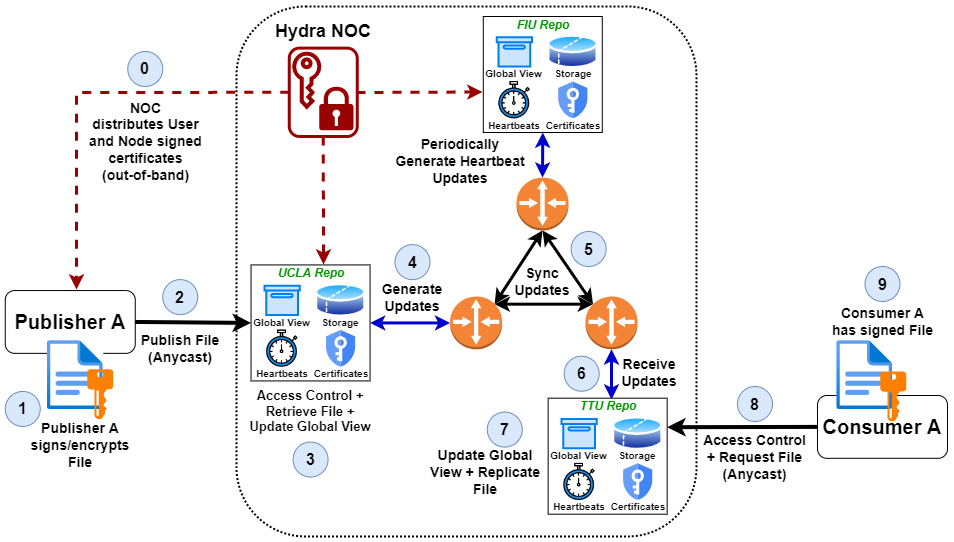
\includegraphics[width=\textwidth]{visuals/overview.png}
    \caption{A High-level overview of Hydra}
    \label{fig:overview}
\end{figure*}

 Figure~\ref{fig:overview} outlines Hydra's general structure along with an overview of the functions performed by Hydra. In its simplest form, a Hydra federation has several geographically distributed nodes and one or more pub-sub groups that allow the nodes to exchange messages among themselves. The Hydra federation also relies on a NOC that is not part of the federation but distributes certificates to the nodes and publishers. 

The process of inclusion of a node into Hydra begins by creating a default route to one of the Hydra nodes and requesting a certificate from the NOC. The NOC authenticates the requests and returns a certificate that the node uses for signing further communication. This completes node bootstrapping. Once the Hydra nodes are bootstrapped and the NOC distributes certificates, a publisher can send an Insert command with a file name \todo{confirm we are NOT using signed Interest}. The command is routed to a Hydra node (decided by NDN routing) that verifies the command and ingests the file. Once the file is ingested, a group message is triggered. Other nodes subscribing to the group message topic receive the notification, update their global view, and some of the nodes start to replicate the file. Each successful replication publishes a group message that allows the nodes to keep track of the degree of replication. The nodes also send out periodic heartbeats to the other nodes so that failure recovery can begin when a node goes offline. Finally, a user or a workflow retrieves a file by sending an Interest with the requested file name to Hydra. This command is routed to a Hydra node that returns the file.
%that authenticates the command, checks if the user is allowed to retrieve the file and returns the file. 
If the file is not available at this node, it sends back a message with a forwarding hint that the application follows to retrieve the file.

\subsection{Naming} \label{sec:naming}
Names in Hydra are important as they are the primary construct of the system.


Hydra uses several types of names:
\begin{itemize}
    \item The Hydra Prefix: decided by the operator(s).\\ Example: \name{/Hydra/}
    \item File (content) Names: decided by data publisher(s). \\Example: \name{/human/genome/dna/hg38}
    \item Node Names: decided by the operator(s).\\ Example: \name{/hydra/node-X1}
    \item The NOC Prefix: decided by operator(s).\\ Example: \name{/hydra/NOC}.
\end{itemize}

%The user facing services are advertised under Hydra's prefix. The File names are independent of this Hydra prefix and as mentioned earlier, can be any NDN name. The prefixes for security operations can be separate or under the Hydra prefix.

%\subsubsection{Hydra Prefix} - include user interface
%\subsubsection{File Names}
%\subsubsection{Node Names} - include forwarding hints
%\subsubsection{NOC Prefix}



\subsubsection{Hydra Prefix}
The <hydra-prefix> acts as the primary namespace for Hydra operations. An example Hydra prefix can be \name{/hydra} or \name{/genomics}. 
This hydra prefix utilizes SVS to actually distribute messages sent on this prefix to all nodes in the federation. %NDN's native anycast capability. We assume  operations can be communicated to any node in the network.

Below are a few more specific uses of sub-namespaces under the Hydra prefix.
\begin{itemize}
    \item \name{/<hydra-prefix>/<function>/<function-info>} is utilized to conduct functions that are user-facing. Users use this prefix for inserting, deleting, and any other interaction that affects data directly within the network. An example might be \name{/hydra/insert/<filename>}.

    \item \name{/<hydra-prefix>/group} is the prefix for group communications. This prefix is utilized for sending messages through State Vector Sync between nodes. The group prefix is under the Hydra prefix since it is used to notify all the nodes of changes in the system.
    
    %The group messaging was created on the <hydra-prefix> due to its importance of providing mass communication for larger needs to the overall network. If this was not on the <hydra-prefix> the SVS protocol would reject the communication or guidance being sent, preventing it from completing its role of notifying network wide changes.
\end{itemize}

\subsubsection{Node prefixes}
The node prefix is utilized for unicast operations which allow Interests to be sent between a specific node and a specific target node within Hydra. The main use case of the node prefix is to enable communication between Hydra nodes. The node prefix is also used for directing a user request to a specific node if the contacted node does not have the content. It is also used for replication.
%Fetching content is utilized for Hydra needs such as replication to the system. Sending an interest for this data would be done through
The node prefix is in the form of \name{/<node-name>/<hydra-prefix>/fetch/...}. This can be appended by operation or content specific names.
% by  content that the node would like to fetch from Hydra. 
%\todo[inline]{clarify this name}

\subsubsection{ForwardingHints}
When data is not present in the node that a user contacted, it returns the name of the node that holds the data. This forwarding hint allows the user to express a subsequent Interest that is steered to a specific node name. 
One example might be \name{/human/genome/dna/hg38} with a forwarding hint to \name{hydra/node-X1}.


%NDN Interests to present a list of names (delegations)
%which are the main use case for naming by allowing users to map any
%provide a pointer to another name. 
%name to any other name. This means that many names can express the same Interest for content such as \name{/genomics/file/example/1} is in reality expressing \name{/hydra/fetch/genomics/file/example/1}. This versatility in naming allows for easy adoption of datasets from other applications.

\subsubsection{Name Prefixes for NOC}
% \todo[inline]{Add these from AlexA's presentation}

NOC is considered the trust anchor of Hydra. While it is not part of the Hydra federation, it uses NDN names for receiving requests. The name prefixes for NOC would be \name{/hydra/NOC/...}.


%\name{/hydra/keys/KEY/...}.

%\pp{I am not sure what other things to add here}

\subsubsection{Node Naming}
%\todo[inline]{There are several assumptions here that need to be reviewed}
%The naming of a Hydra node is not immediately apparent as there are limitations and advice to be utilized when deciding a name. The limitations ordinate from our data distribution protocol, SVS, which may be improved or changed in the future for the longevity of Hydra. Nevertheless, these limitations should always be heavily considered when creating node names.

%A short name (<= 20 characters) is almost necessary for %Hydra as long names limit the number of nodes able to join Hydra. SVS's sync interests which contain all node names have an innate problem with the maximum size of an NDN interest. Due to our modifications of SVS, we do handle the case where the sync interest is too large to be a valid NDN interest. However, this increases network overhead so it should be avoided. As such, we strongly recommend that all names contain 20 characters or less to ensure Hydra can include a decent amount of nodes which is extremely important for long term usage.

Nodes names are required to be unique. Hydra does not add any extra components to a node name when using it for communication. 
%This is not only because of the space limitation but also because the node names should make an attempt to precisely describe the node. %From the fact of being an NDN application, there is not an IP address indicating the exact system of a node. Therefore, the name of a node naturally produces merit when chosen carefully. Examples of good 
Example names can be
%are the following:
\name{'/TnTech/CSC/hydra'} or \name{'/hydra/node-xx'}, or \name{'/norm-labs/hydra-5'}.


\subsubsection{Certificate names}
Hydra uses a hierarchy of certificate names to provide trust. 

An example Hydra root key (hydra root = hydra trust anchor) would be \name{/hydra/KEY/…}.

Node cert names can be \name{/hydra/32=nodes/host.ucla/KEY/… (key for UCLA node)} or 
\name {/hydra/32=nodes/fabric-hostXYZ/KEY/… (key for hostXYZ)}.

The user cert names can be  \\
\name{/hydra/32=users/XX@gmail.com/32=ns/FIU/experiments/KEY/...} or 
\\
\name{/hydra/32=users/YY@gmail.com/32=ns/FIU/experiments/2022/KEY/...}



\subsubsection{Content naming}
There are two ways we can name files in Hydra. First, we can utilize the content names created by the publisher. Example of such a name would be \name{/human/genome/dna/hg38}. The other option is to utilize Hydra specific names such as \name{/hydra/human/genome/dna/hg38}. While both are acceptable, there are a few trade-offs. With the first option, we assume the owner of the name prefix (i.e., \name{/human/genome} will allow Hydra to announce the prefix. Second, if publishers publish content using different name prefixes, a Hydra node must announce all those name prefixes into the routing system (e.g. \name{/human/genome} and \name{/kidney}). Finally, creating an easy-to-utilize trust schema that might be difficult. \too{verify}. On the other hand, appending the \name{/Hydra} prefix to each name makes trust relations and routing announcements simpler. A node can simply announce the \name{/Hydra} prefix into the routing system. However, this requires changing the content names (e.g./ \name{/human/genome/dna/hg38} becomes \name{/hydra/human/genome/dna/hg38}, which makes the content specific to the Hydra framework. For our implementation, we use the first naming model.\todo{verify}.
 % needs work

\subsection{Functions} \label{subsec:functions}

\begin{figure*}[!ht]
    \centering
    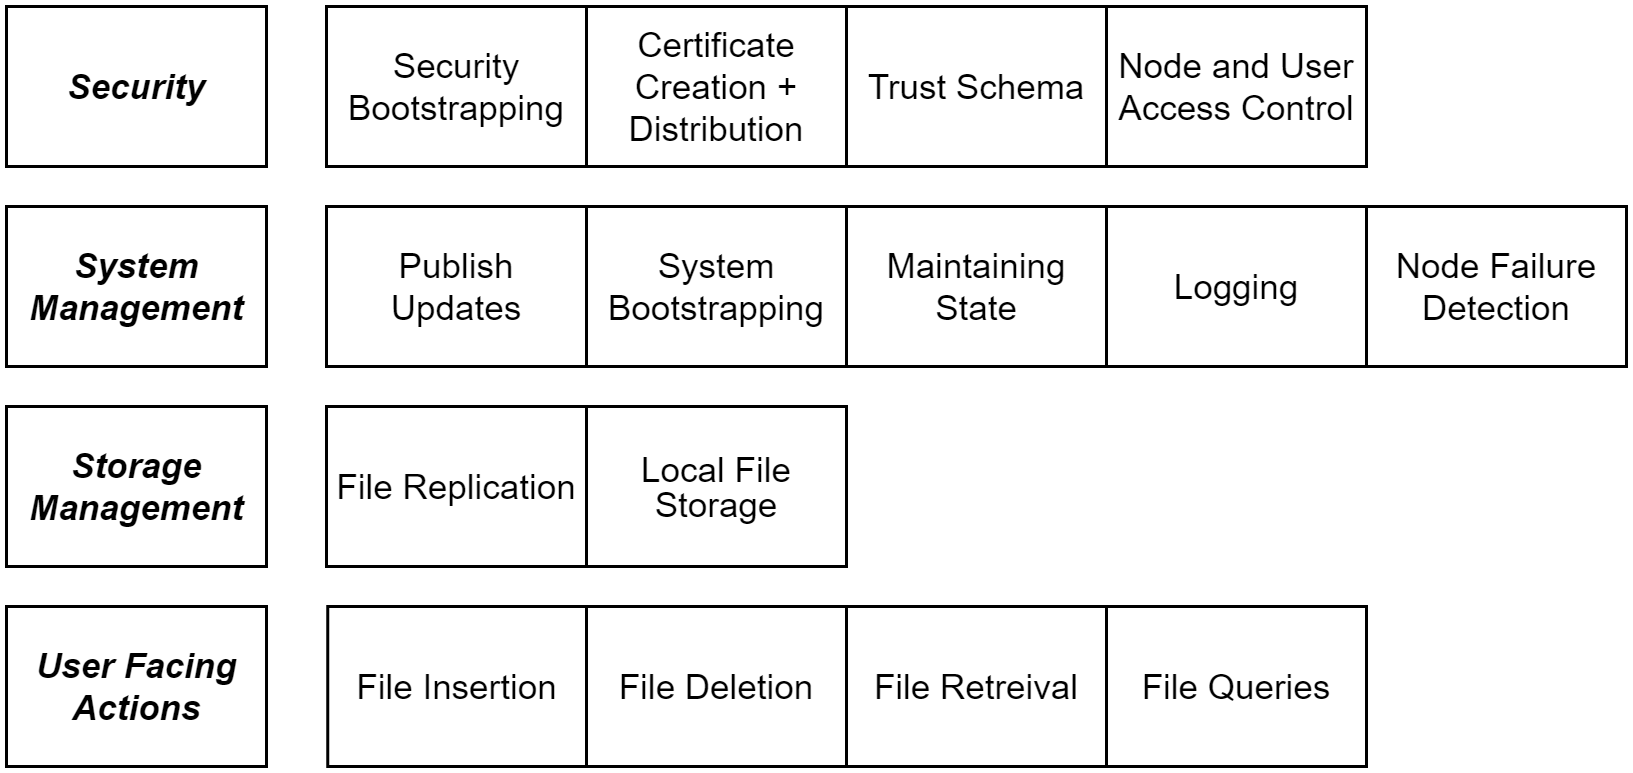
\includegraphics[width=2\columnwidth]{visuals/node-functions.png}
    \caption{Necessary Functions of a Hydra Node}
    \label{fig:node-functions}
\end{figure*}
%\todo[inline]{This needs to be updated. Remove the lines, and make sure the boxes are correct. - Justin}

As Figure~\ref{fig:overview} outlines, a Hydra federation has four types of functions:

\begin{itemize}
    \item Bootstrapping
    \item System Management
    \item Storage Management
    \item User Facing Functions
\end{itemize}

Figure~\ref{fig:node-functions} outlines each of these categories.
%and what exact functions go into them. An explanation of these categories and further references follow.

\subsubsection{Bootstrapping} can be divided into security bootstrapping and system bootstrapping. Security bootstrapping focuses on getting proper key and certificate information that the node can present to the federation before it is allowed to join. We discuss bootstrapping in Section   \ref{sec:node-operations}. System bootstrapping focuses on the functionality needed for a new node to join the federation and sync the node's state to the system's state. 

\subsubsection{System Management} modules provide the necessary systems level functionality for Hydra. These include maintaining states in the network, publishing and applying updates to the system state, 
% user access control (NOTE: this should go to security), 
logging, node failure detection, and failure recovery. These functions are at the core of how Hydra operates. Management of system is discussed further in Section \ref{sec:node-operations}.

\subsubsection{Storage Management} functions oversee file replication and local file storage. The file replication module replicates files across Hydra nodes and maintains the degree of replication (currently 3). This ensures data loss does not occur even when individual nodes fail. The local file storage module handles the storage functions of a node. These include interacting with the underlying database or filesystem, and freeing up storage by deleting unused files.
%Both functions are necessary for maintaining copies of uploaded files throughout the system, ensuring data is not lost. 
Further discussion on file replication can be found in Section \ref{sec:data-operations} and local storage can be found Section \ref{subsec:modules}.

\subsubsection{User Facing functions} provide user interfaces for various user and application interactions. These functions include file insertion, deletion, retrieval, and system status checks. Hydra exposes name-based APIs for these functions that can be directly used by the users or integrated into separate applications. More details on user facing functions can be found in Section \ref{sec:data-operations}.
\subsection{Modules} \label{subsec:modules}
\begin{figure}[!ht]
    \centering
    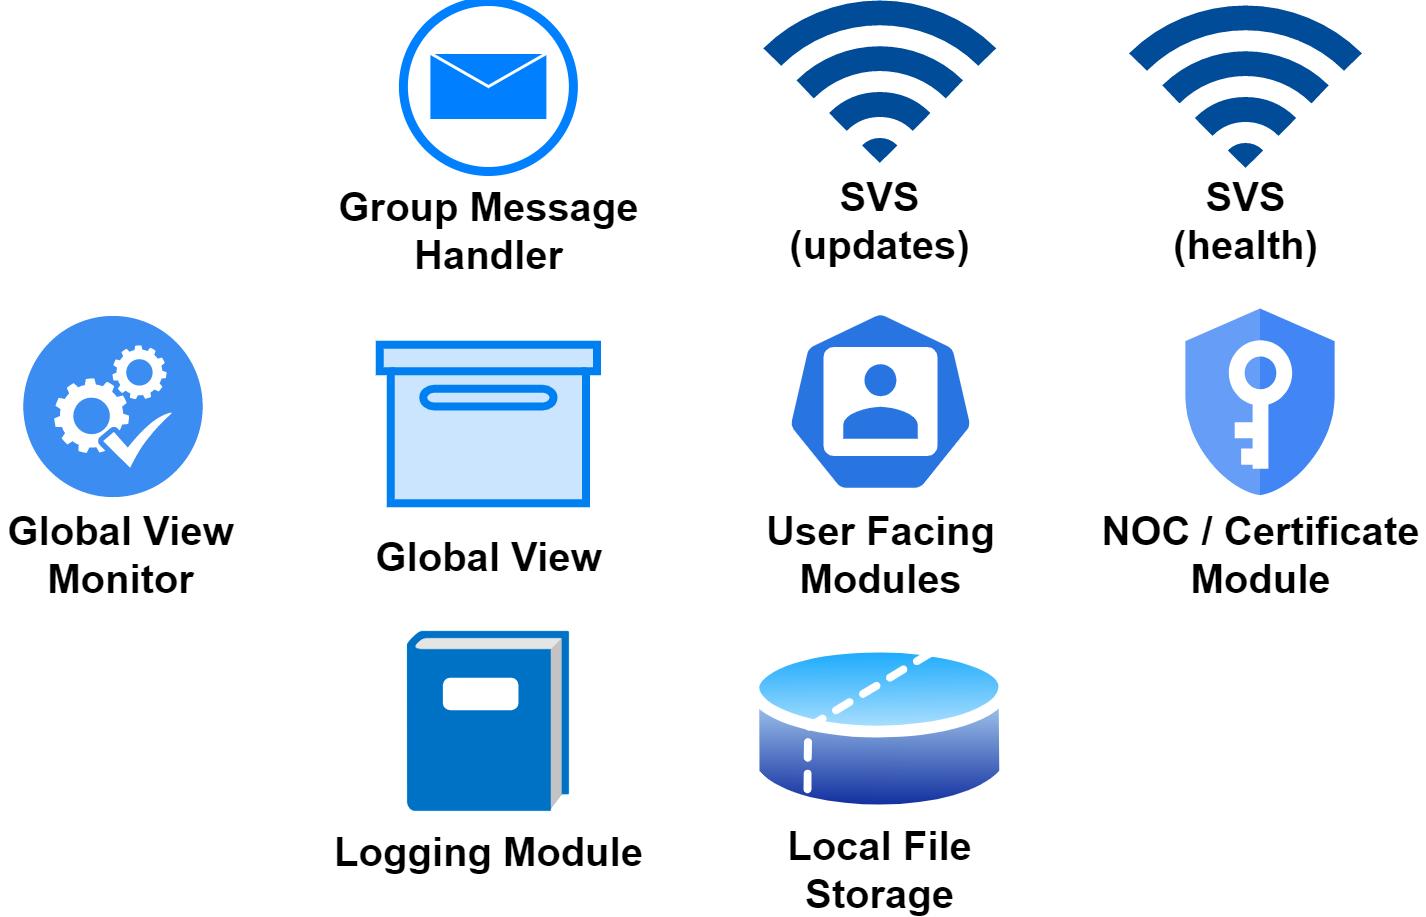
\includegraphics[width=\columnwidth]{visuals/node-modules.png}
    \caption{Modules that make up a Hydra Node}
    \label{fig:node-modules}
\end{figure}
%\todo[inline]{Lixia says - heartbeat tracker should be part of the global view monitor}

To provide the functions described in Subsection~\ref{subsec:functions}, a Hydra node is made up of several modules as illustrated in  Figure~\ref{fig:node-modules}. Nine modules make up a Hydra node, and the following list briefly describes each of them. 
%More information will be later explained further in the paper.

%\subsubsection{Heartbeat Tracker}
%The heartbeat tracker is a module in a Hydra node that a node uses to track all other nodes in the system. Each node sends a heartbeat every 30 seconds that is propagated using group messaging (SVS - see Module below) to all the other nodes. If a node X does not hear a heartbeat message from another node Y, it presumes node Y is unreachable and sets the node in the heartbeat tracker to ``Unreachable". 
%If a node comes back online after failure, it sends out a heartbeat message and node X sets node Y to be ``Alive"  in the heartbeat tracker.
%Heartbeat Tracker interacts with Global view, and Group message handler. 

%of all nodes within Hydra and periodically send out a heartbeat of its own.

\subsubsection{StateVectorSync (SVS)}
%The SVS protocol is used for the exchange of group messages between all nodes within Hydra (group messages - see Section 4.1). SVS will update node states, notifying other nodes of recent changes via Group Messages(GMs), which helps maintain a consistent view across nodes.  As mentioned above, SVS interacts with group messages.

The SVS module uses the SVS protocol to publish data (e.g., state update messages) that is received by all other nodes within Hydra. SVS allows Hydra to maintain a consistent view across the nodes.

\subsubsection{Global View}
%The global view contains complete information about the Hydra system, including all node information, all files and, for each \emph{file}, which nodes own and take over the file, as well as meta-info such as size, origin node, numbers of copy, etc (global view - see Section 4.4). Global View Monitor is only used to monitor the global view. Without the global view monitor, no node would do anything that supports other nodes. The monitor constantly checks the global view (which is constantly updated) and finds out what it needs to do, for example if it needs to fetch/store files.
The Global View is a local database to a Hydra node. It represents a node's view of the Hydra federation. The global view contains information related to the Hydra system such as files' metadata, node information, and replication information.

It also contains the heartbeat tracker sub-module that is used to send and track a heartbeat message. The heartbeat message establishes whether a node is alive or unavailable.  If the nodes in the federation do not hear a heartbeat message from a node for a certain time, it presumes the node is unreachable and sets the node in the heartbeat tracker to ``Unreachable". Once $n$ heartbeats are missed from a specific node, the nodes initiate automatic replication.



%and all files' metadata.


\subsubsection{Group Message Handler}
%All processes join a ``group" via SVS and synchronize the global view by publishing group messages. Group messages posted by a node are visible to all nodes, just like chatting in a group. Naturally, Group Message Handler interacts with SVS and Group messages.(group messages handler - see Section XX)

All Hydra nodes join a ``group" via SVS and synchronize the global view by publishing group messages. Group messages posted by a node are visible to all nodes. This module handles Group Messages - messages that are sent to the group of Hydra nodes. The group message handler interacts with SVS to receive and apply the new updates to Global view and publish new group messages.
%them and appropriately affecting the Hydra node based on them.


\subsubsection{Global View Monitor}
%This module constantly checks the global view (which is constantly updated) and finds out what the Hydra node needs to fetch or store.
The global view monitor monitors the global view database for any changes. If a change is detected, it initiates an outgoing update message. It also applies update messages received by the node to the Global view database.

\subsubsection{User-Facing Modules}
%The features within the hydra system that are available to users, including insert, delete, query, and retrieval. 
%When a node receives an Insertion command for a file, the node first correctly authenticates the command and then immediately starts fetching the file. When the file is stored, the node forms an "insert" GM and applies this GM to its global view (insertion - see Section 5.1).
%When a node receives a Deletion command, if the node has the file or a copy of this file, it deletes the file or the copy. The GM "delete" is generated by deleting the file to update its global view.(deletion - see Section 5.4).
%When a node receives a Query command, the node simply checks the query type information in the global view and returns it via packet. (querying - see Section 5.4).
%When a node receives a Retrieval command, there are 3 possible scenarios. (1) Hydra does not have the file; (2) The node does not have the file, but another node does; (3) The node has the file (retrieval - see Section 5.3).

These public-facing modules allow users to interact with the Hydra system, providing data insertion, deletion, and retrieval functionality. They also allow the user/applications to query the system for file availability. 

\subsubsection{Network Operation Center (NOC)}
%Acts as the system trust anchor for Hydra deployments, and issues the certificate. A new Hydra node fetches a trust anchor by sending an Interest and verifies the returned self-signed certificate out-of-band. Then the node signs the Interest and requests a certificate from the NOC. Finally, NOC signs the certificate using the trust anchor and returns it in the replied data. 
NOC is a centralized entity that acts at the root of trust for a deployment. NOC provides signed certificates to the nodes and users. %and key information in order be apart of the system.

\subsubsection{Logging Module}
%Enable logging globally for the entire hydra system to monitor and troubleshoot errors for easy optimization.

This module logs all node records (data operations and errors) to monitor Hydra and provide information to the administrator.

\subsubsection{Local File Storage}
%It's the module that writes files to the actual file system, garbage collects, and interfaces with Insertion/Deletion/Querying/Replication/Retrieval modules. It is also closely related to the storage size.
Local file storage is the Database on a node that holds the Data packets corresponding to a published file. The file storage module also performs garbage collection and deletes any file not accessed for a certain duration.
%This database stores the files that the Hydra node said it would store.
% \section{The Hydra Specification} \label{sec:specification}

% This section describes the entire Hydra specification in detail.

\subsection{Files} \label{sec:files}
Hydra uses the term \emph{file} to describe the data unit of insertion, deletion, retrieval, or replication. However, a file is not necessarily a file in the UNIX system; it is just a BLOB of data that is identified by a unique name. See Section~\ref{sec:naming} for more details on file names.

A file consists of NDN Data packet(s); however, the size of a file directly impacts the performance of the following operations: replication, failure recovery, insertion, and retrieval. These NDN Data packet(s) also determine the unit size of a particular file.

%\jcp{is this following paragraph right? should we leave this access control out since its going to be in Hydra 0.3?}

%Hydra is simply a holder of files as the data publisher's signature is maintained since its creation. Hydra provides access control by encrypting a file's NDN Data packet and creating a new signed NDN Data packet with the previously encrypted NDN Data packet as the content. See Section~\ref{sec:security} for more details on security and access control. % good
\subsection{Favor} \label{sec:favor}
Due to Hydra being a federation of storage nodes with different storage capacities and policies, it is necessary to have a mechanism that can express a node's local conditions and preferences for storing or replicating additional files.

\textit{Favor} can be thought of as "how suitable a node is to carry file(s)".
Every node is responsible for calculating a numeric value for node X where X is each node within the system including itself. The range of this numeric value is determined by the formula used. As implicitly indicated, favor is an entirely local calculation. However, all parameters of the calculation are announced by every node giving each node complete control over what and which files are stored in their respective storage. Essentially, favor protects node independence within the federated system.

As it stands, favor is calculated per node and all parameters are included in every GM in order to be as up to date as possible. To limit network traffic, Hydra does not send a GM when these parameters change. See Section~\ref{sec:group-messages} for more details on GMs.

Favor calculations may incorporate the following aspects:
\begin{itemize}
    \item storage capacity (current usage and max usage)
    \item network stability / traffic
    \item location
    \item prefix preferences, file origin, node's labels, etc
    \item local policy
\end{itemize}

Favor affects Hydra's overall performance, usability, and stability. For our initial implementation, we simplified favor's calculation to be based only on storage capacity.

In the future, additional parameters and functions of favor may be necessary for different applications. For example, a baseline favor value may be necessary for high-volume storage environments to reserve some capacity for file takeovers essentially protecting Hydra's resiliency. See Section~\ref{sec:future-work} for more details on future work. % good
\subsection{Storage} \label{sec:storage}
A Hydra node utilizes several databases for maintaining state and for storage of different types of data.

Each of these databases is described briefly below.
\begin{itemize}
    \item SVS Database: A database of all published messages over the Sync group, implemented as a key-value store.
    \item Global View: A Hydra node's state -- a relational database containing all information relating to the entire system.
    \item Local File Storage: A key-value database holding files that the Hydra node is storing.
    \item Local Reserved Storage: A sectioned off part of Local File Storage to only be used to help with special operations such as data ingestion. This space is not used for storing replicated files or Hydra's metadata.
    \item Command Table: A table holding the progress and status of the commands being currently executed.
    \item Logs: These may either be stored locally or inside a distributed logging system or both.
    \item Certificate and Key Database: A key-value database that holds key and certificate information required for secured publication of messages, data validation, and user authentication.
\end{itemize}

Currently, we do not impose any limit on these storages. However, operational deployments will need to define the storage limit for these databases. % needs work
\subsection{StateVectorSync Protocol} \label{sec:svs}

Since Hydra is a distributed system, a distributed dataset synchronization (Sync) protocol is required to keep the global view synchronized, by communicating events such as file insertions, deletions or failures to all other nodes. Hydra uses the State Vector Sync (SVS) protocol\cite{} to achieve efficient and loss resilient global view synchronization.
SVS is further discussed in Subsection~\ref{sec:svs}.

While GMs help exchange states, we still need a way to transfer and synchronize GMs between hosts. For this purpose, Hydra utilizes the State Vector Sync (SVS) protocol. %will be leveraged for message propagation between repo nodes. 
Note that this sync protocol only provides eventual consistency guarantees. Note that SVS only provides a pub-sub capability for message exchange. Hydra is able to utilize any other pub-sub system for message exchange.

%Conveniently for us, there was a Distributed Dataset Synchronization Protocol survey published that outlines multiple current solutions for doing this\cite{}

%\jcp{mention distributed dataset syn. protocols and include the survey paper}
 % needs work
\subsection{Group Messages} \label{sec:group-messages}
%In a distributed system, the existence of a message protocol 
%smoothies communication between nodes allowing the system to act as one entity. 
%Hydra is no different and operates using 'Group Messages' (GMs). 
Hydra utilizes Group Messages (GMs) to exchange updates among nodes.
A published Group Message goes out to every node within Hydra such that every node receives every Group Message. %The philosophy behind this is that nodes can act in a more precise and knowledgeable way knowing all past actions within Hydra.
Understanding  all past actions in Hydra allows the nodes to act in a more precise and knowledgeable manner.

There are six Group Message types with each performing different actions. %These messages are used for  having different effects within the system:
\begin{itemize}
    \item Insert: a GM containing metadata of a new file that is inserted in Hydra.
    \item Delete: a GM containing information about a file to delete from Hydra.
    \item Claim: a GM stating the node is going to fetch or is unable to fetch a certain file.
    \item Store: a GM stating a node has stored a file in its local storage. %information needed to know that a node stored a file.
    \item Heartbeat: a GM that is periodically published by nodes to let others know that it is alive. In our current implementation, the interval of heartbeats is set to 30 seconds. %maintain a soft state.
    \item Correct: a GM to correct a local storage v.s. system information mismatch, used by previously failed nodes. \todo[inline]{Susmit - don't remember discussing this}
    \item Leave: a GM send by a leaving node in order to help speed up replication
\end{itemize}

To keep network overhead low, we treat all messages as heartbeat messages. If there is no GM withing a specified time, a specific heartbeat message is announced.
%Our distributed dataset  synchronization protocol will likely be expensive on a network. Therefore to help tackle this, every GM is technically a Heartbeat GM to limit GM traffic. % needs work
\subsection{Global View} \label{sec:global-view}
The Global View can be thought of as %"what a node views the entire system as".
a node's view of the entire system.

As nodes exchange messages (Group Messages, see next section), a Hydra node creates and stores the state of the system in a light-weight local database known as the 'Global View'. 

%With every node receiving every Group Message, Hydra needs a way for nodes to store that information. Rather than storing raw Group Messages, Hydra stores the effects of each Group Message along with any relevant information in a light-weight local database known as the 'Global View'. 

Note that this Global View is not stored once in a global storage accessible by every node. Instead, each node has its own version of this global view that they maintain. Throughout the duration of operation, a Hydra node synchronizes this database with the other nodes through continuously published group messages.

%and is constantly checked for possible actions to be taken by the node.

Every node in Hydra has a global view of:
\begin{itemize}
    \item All node information
    \item Each file’s specifics
    \begin{itemize}
        \item which nodes are in possession of the file (the “on list”)
        \item which nodes can step up to take over the file (the “backup list”)
        \item meta-info (size, origin node, copies, and etc)
    \end{itemize}
\end{itemize}

The Global View also has the ‘state vector’ that made up the Global View. This state vector is the same type found in SVS and indicates the sequence of messages that were incorporated into the state.

Global View layout example (capital alphabetical letters are placements for node names):
{\small
\begin{spverbatim}{
"state_vector": {"A":123,"B":120,"C":100,"D":150,"E":123},

"nodes": [
    {"name": "D", "favor": 50, “alive”: True},
    {"name": "C", "favor": 20, “alive”: True},
    {"name": "B", "favor": 15, “alive”: True},
    {"name": "A", "favor": 10, “alive”: True},
    ...
    ],

"files":[
    {
        "name": "/genomics/fileA",
        "size": 128,
        "contact": "B",
        "copies": 3,
        "on": ["B","A","D"],
        "on_history": ["C"]
    },
    ...
    ]
}\end{spverbatim}
} % needs work
\subsection{PubSub Protocol} \label{sec:pubsub}

% this is a temp paragraph, will expand it later
Hydra's interface for data insertion and data deletion takes inspiration from the previous incarnation of standalone NDN repo\cite{}. A PubSub-like protocol is used for exchanging messages with clients such as file insertion commands and updates. These operations are further outlined in Section~\ref{sec:data-operations}. % needs work
\subsection{Command Structures} \label{sec:command-structures}

\jcp{TODO: FirstContact, NotificationSpecification, etc PubSub structs}

 % needs work
\subsection{Status Codes} \label{sec:status-codes}

Users can receive multiple status codes (like a server error + redirection for instance), the following is an overview of all status codes in Hydra. 

% Used the following table by: https://www.tablesgenerator.com/
\begin{table}[]
\caption{Hydra Command Status Codes}
\begin{tabular}{|cc|}
\hline
\multicolumn{1}{|c|}{\textbf{Status}}   & \textbf{Code} \\ \hline
\multicolumn{2}{|c|}{\textbf{Informational}}            \\ \hline
\multicolumn{1}{|c|}{STAND\_BY}         & 100           \\ \hline
\multicolumn{1}{|c|}{FETCHING}          & 101           \\ \hline
\multicolumn{2}{|c|}{\textbf{Success}}                  \\ \hline
\multicolumn{1}{|c|}{OK}                & 200           \\ \hline
\multicolumn{2}{|c|}{\textbf{Redirection}}              \\ \hline
\multicolumn{2}{|c|}{\textbf{Client Error}}             \\ \hline
\multicolumn{1}{|c|}{BAD\_NAME}         & 400           \\ \hline
\multicolumn{1}{|c|}{BAD\_REQUEST}      & 401           \\ \hline
\multicolumn{1}{|c|}{UNAUTHENTICATED}   & 402           \\ \hline
\multicolumn{1}{|c|}{UNAUTHORIZED}      & 403           \\ \hline
\multicolumn{1}{|c|}{NOT\_FOUND}        & 404           \\ \hline
\multicolumn{1}{|c|}{NO\_COMMAND}       & 405           \\ \hline
\multicolumn{2}{|c|}{\textbf{Server Error}}             \\ \hline
\multicolumn{1}{|c|}{RESOURCE\_LIMIT}   & 500           \\ \hline
\multicolumn{1}{|c|}{TRAFFIC\_OVERLOAD} & 501           \\ \hline
\multicolumn{1}{|c|}{NODE\_DISCONNECT}  & 502           \\ \hline
\multicolumn{1}{|c|}{UNKNOWN\_ERROR}    & 503           \\ \hline
\end{tabular}
\label{tab:status-codes}
\end{table} % needs work
%\section{Security - Alex/Proyash/Tianyuan} \label{sec:security}

Acts as the system trust anchor for Hydra deployments, and issues security certificates. A new Hydra node fetches a certificate by sending an Interest. Next the node verifies the returned self-signed certificate out-of-band. Then the node signs the Interest and requests a certificate from the NOC. Finally, NOC signs the certificate using the trust anchor and returns it in the replied data.




In order to authenticate the Hydra group communications and interactions with users, Hydra’s security model includes three roles in the system.
\begin{itemize}
\item Network Operator Center (NOC): serving as the system trust anchor for each Hydra deployment, adding or deleting Hydra nodes from the federation, and managing the security policies for the Hydra system.
\item Hydra Node: a server that joins the federated repo system. One trusted server might start a new process if the old one terminates.
\item Client: users who use the Hydra system by sending Insertion and Deletion commands or data requests.
\end{itemize}

In Hydra’s security design, we assume the NOC is trusted, and each Hydra node is also trusted once added. To bootstrap one Hydra node to the system, out-of-band verification (e.g., pre-shared passcode, email verification) is needed to authenticate the initial communication between the Hydra node and NOC. A new Hydra node fetches the trust anchor by sending Interest /hydra/bootstrap/anchor, and verifying the returned self-signed certificate out-of-band. Then it uses the out-of-band pre-shared material to sign Interest /hydra/bootstrap/cert and request a certificate from the NOC. Verifying the certificate requester’s authenticity, the NOC uses the trust anchor to sign a certificate and returns it in the replied Data. The new Hydra node learns its node name from the certificate via certificate installation. After installing the trust anchor and node certificate, the Hydra node keeps its security policies up-to-date by periodically send Interest /hydra/bootstrap/schema and fetch new policies.
\\The Hydra group communication should also be protected from invalid message senders. Therefore, Hydra requires each node to sign the Interest and Data in group communication and enforce the system membership checking through verifying the signer’s certificate with the trust anchor.
\\Besides that, users’ commands to the Hydra system should also be authenticated. Different from authenticating the group communication among Hydra nodes, Hydra users do not share the trust anchor with the Hydra nodes. The identity of users can only be verified along the certificate chain when the Hydra nodes have users’ trust anchors. Hydra achieves this via security policy distribution, where individual Hydra nodes fetch the trusted anchors and corresponding signing rules under those namespaces. // SECURITY STUFF ADD % needs work